\documentclass[lettersize,journal,onecolumn]{IEEEtran}
\usepackage{amsmath,amssymb,amsfonts}
\usepackage{booktabs,multirow,array,tabularx}
\usepackage{graphicx}
\usepackage{xcolor}
\usepackage{url}
\usepackage{cite}
\usepackage{algorithm}
\usepackage{algpseudocode}
\usepackage{graphicx}
\usepackage{textcomp}
\usepackage{balance}
\usepackage{hyperref}
\hypersetup{colorlinks=true,linkcolor=blue,citecolor=blue,urlcolor=blue}

\graphicspath{{supplement_figs/}{../results/figures/}}

\begin{document}

\title{Supplemental Material for\\
``Constrained Binary Subset Selection under Interval Boxes:\\
A Fair-Budget Benchmark with Application to Food Assembly''}

\author{Lei~Zhao, Fujin~Huang, Xinning~Liu, Li~Han, Ling~Kang, and Quan~Guo}

\maketitle
\pagenumbering{arabic}
\renewcommand{\thepage}{S\arabic{page}}
\renewcommand{\thetable}{S\arabic{table}}
\renewcommand{\thefigure}{S\arabic{figure}}
\renewcommand{\theequation}{S\arabic{equation}}
\setcounter{page}{1}
\setcounter{table}{0}
\setcounter{figure}{0}

\begin{abstract}
The source code, raw run CSVs, and reproduction scripts are publicly available at the project repository
(\url{https://github.com/tyrone1979/nutri-range-opt-survey/}).
This supplemental document therefore does \emph{not} reproduce code listings.
Instead, it provides detailed instance configurations, extended statistical tables, post-hoc significance tests,
diagnostic plots for abandoned exploratory analyses, and cell-by-cell Feasible Hit Rate (FHR) breakdowns that
complement the PRIMARY results in the main manuscript.
\end{abstract}

\section*{Scope and Notation}
Unless stated otherwise, all PRIMARY campaigns use population size $500$, evaluation ceiling $100{,}000$,
ten hashed seeds, and the same RCFA decode/feasibility predicate as in the main manuscript.
FHR cells below report \emph{seed-level} mean$\pm$std: within each seed we average FHR over the twelve representative targets,
then compute mean and standard deviation across the ten seeds.
Pairwise tests (Part~D) are Wilcoxon signed-rank tests paired by $(\mathrm{target},\mathrm{seed})$.
Throughout, ``Table~$k$ / Fig.~$k$ of the main manuscript'' refers to the camera-ready main paper;
local numbering uses the prefix~S.

\section{Part A: Detailed Benchmark Instance Construction}
\label{sec:sa}

PRIMARY does \emph{not} use a single fixed DRI box for all runs.
Instead, it uses twelve NHANES-derived representative targets stored in
\texttt{data/representative\_targets.csv}.
Each target activates a subset of the canonical nutrient vocabulary
(union size~$15$ across the twelve targets; NHANES food matrix has sixteen nutrient columns).
Table~\ref{tab:s1} lists every active nutrient interval $(L_j,U_j)$ for each representative.
Sentinel uppers $U\!\ge\!10^{5}$ (e.g., saturated fat) are treated as one-sided constraints and replaced by
empirical meal-total caps before width scaling (main manuscript Eq.~(5) and E2 protocol).

\begin{table}[!t]
\centering
\caption{Complete nutrient interval boxes for PRIMARY representatives \texttt{rep\_000}--\texttt{rep\_005}.
Values are taken verbatim from \texttt{target\_json}; $U=10^{7}$-scale entries denote sentinel/one-sided uppers.
Representatives \texttt{rep\_006}--\texttt{rep\_011} appear immediately below as a non-floating continuation.}
\label{tab:s1}
\scriptsize
\begin{tabular}{@{}clrr@{}}
\toprule
Target & Nutrient & $L_j$ & $U_j$ \\
\midrule
rep\_000 & calcium & 1200 & 2000 \\
 & calorie & 1400 & 2300 \\
 & carb & 200 & 350 \\
 & cholesterol & 0 & 300 \\
 & potassium & 2600 & 5000 \\
 & protein & 0 & 50 \\
 & saturated\_fat & 0 & $10^{7}$ \\
 & sodium & 0 & 1500 \\
 & vitamin\_c & 75 & 2000 \\
 & vitamin\_d & 20 & 100 \\
\midrule
rep\_001 & calorie & 1800 & 3400 \\
 & carb & 300 & 550 \\
 & cholesterol & 0 & 200 \\
 & fiber & 31 & 99999 \\
 & potassium & 3400 & 5000 \\
 & protein & 0 & 70 \\
 & saturated\_fat & 0 & 25 \\
 & sodium & 0 & 1500 \\
\midrule
rep\_002 & calcium & 1000 & 2500 \\
 & calorie & 1700 & 3300 \\
 & carb & 300 & 500 \\
 & cholesterol & 0 & 300 \\
 & potassium & 3400 & 5000 \\
 & protein & 0 & 60 \\
 & saturated\_fat & 0 & $10^{7}$ \\
 & sodium & 0 & 1500 \\
 & vitamin\_c & 90 & 2000 \\
 & vitamin\_d & 15 & 100 \\
\midrule
rep\_003 & calorie & 1900 & 3500 \\
 & carb & 300 & 550 \\
 & cholesterol & 0 & 300 \\
 & potassium & 3400 & 5000 \\
 & protein & 0 & 70 \\
 & saturated\_fat & 0 & $10^{7}$ \\
 & sodium & 0 & 1500 \\
\midrule
rep\_004 & calorie & 0 & 3300 \\
 & carb & 300 & 500 \\
 & cholesterol & 0 & 300 \\
 & protein & 0 & 80 \\
 & saturated\_fat & 0 & 20 \\
 & sugar & 0 & 25 \\
\midrule
rep\_005 & calorie & 0 & 4900 \\
 & carb & 450 & 750 \\
 & cholesterol & 0 & 300 \\
 & potassium & 3400 & 5000 \\
 & protein & 0 & 110 \\
 & saturated\_fat & 0 & 30 \\
 & sodium & 0 & 1500 \\
 & sugar & 0 & 36 \\
\bottomrule
\end{tabular}

\end{table}

\noindent\textbf{Table~\ref{tab:s1} (continued).}
Nutrient interval boxes for representatives \texttt{rep\_006}--\texttt{rep\_011}.\\[0.4em]
{\centering\scriptsize\begin{tabular}{@{}clrr@{}}
\toprule
Target & Nutrient & $L_j$ & $U_j$ \\
\midrule
rep\_006 & calorie & 1600 & 3100 \\
 & carb & 300 & 500 \\
 & cholesterol & 0 & 300 \\
 & folic\_acid & 400 & 1000 \\
 & iron & 8 & 45 \\
 & protein & 0 & 60 \\
 & saturated\_fat & 0 & $10^{7}$ \\
 & vitamin\_b12 & 0 & 2.4 \\
 & vitamin\_c & 90 & 2000 \\
\midrule
rep\_007 & calorie & 0 & 3000 \\
 & carb & 250 & 450 \\
 & cholesterol & 0 & 300 \\
 & fiber & 25 & 99999 \\
 & potassium & 2600 & 5000 \\
 & protein & 0 & 60 \\
 & saturated\_fat & 0 & 20 \\
 & sodium & 0 & 1500 \\
 & sugar & 0 & 25 \\
\midrule
rep\_008 & calorie & 2100 & 3600 \\
 & carb & 350 & 550 \\
 & cholesterol & 0 & 300 \\
 & fiber & 38 & 99999 \\
 & protein & 60 & $10^{7}$ \\
 & saturated\_fat & 0 & $10^{7}$ \\
 & sodium & 0 & 1500 \\
 & sugar & 0 & 36 \\
\midrule
rep\_009 & calorie & 0 & 2900 \\
 & carb & 250 & 450 \\
 & cholesterol & 0 & 300 \\
 & fiber & 21 & 99999 \\
 & protein & 70 & $10^{7}$ \\
 & saturated\_fat & 0 & 20 \\
 & sodium & 0 & 1500 \\
 & sugar & 0 & 25 \\
\midrule
rep\_010 & calorie & 0 & 2900 \\
 & carb & 250 & 450 \\
 & cholesterol & 0 & 200 \\
 & fiber & 21 & 99999 \\
 & potassium & 2600 & 5000 \\
 & protein & 0 & 70 \\
 & saturated\_fat & 0 & 20 \\
 & sodium & 0 & 1500 \\
 & sugar & 0 & 25 \\
\midrule
rep\_011 & calorie & 0 & 4300 \\
 & carb & 400 & 650 \\
 & cholesterol & 0 & 300 \\
 & fiber & 31 & 99999 \\
 & potassium & 3400 & 5000 \\
 & protein & 90 & $10^{7}$ \\
 & saturated\_fat & 0 & 30 \\
 & sodium & 0 & 1500 \\
 & sugar & 0 & 36 \\
\bottomrule
\end{tabular}
\par}

Table~\ref{tab:s2} shows how width factor $f\in\{0.5,1.0,1.5\}$ transforms the sanitized box of
\texttt{rep\_000} under the PRIMARY sparsity operator (finite dimensions: center scaling;
unbounded dimensions: one-sided cap scaling).
Decreasing $f$ contracts finite faces and is the geometric mechanism behind the large absolute FHR gap in E2.

\begin{table}[!t]
\centering
\caption{Sparsity scaling example for \texttt{rep\_000}.
Columns $L^{0},U^{0}$ are the sanitized reference box at $f=1.0$;
$L(f),U(f)$ are the PRIMARY operator outputs at $f=0.5$ and $f=1.5$.
Caps for sentinel dimensions use the E2 sanitization rule (not a hand-tuned DRI table).}
\label{tab:s2}
\scriptsize
\begin{tabular}{@{}lrrrrrr@{}}
\toprule
Nutrient & $L^{0}$ & $U^{0}$ & $L(0.5)$ & $U(0.5)$ & $L(1.5)$ & $U(1.5)$ \\
\midrule
sodium & 0.0 & 1500.0 & 375.0 & 1125.0 & 0.0 & 1875.0 \\
potassium & 2600.0 & 5000.0 & 3200.0 & 4400.0 & 2000.0 & 5600.0 \\
calorie & 1400.0 & 2300.0 & 1625.0 & 2075.0 & 1175.0 & 2525.0 \\
protein & 0.0 & 50.0 & 12.5 & 37.5 & 0.0 & 62.5 \\
carb & 200.0 & 350.0 & 237.5 & 312.5 & 162.5 & 387.5 \\
saturated\_fat & 0.0 & 5000.0 & 0.0 & 2500.0 & 0.0 & 7500.0 \\
cholesterol & 0.0 & 300.0 & 75.0 & 225.0 & 0.0 & 375.0 \\
calcium & 1200.0 & 2000.0 & 1400.0 & 1800.0 & 1000.0 & 2200.0 \\
vitamin\_d & 20.0 & 100.0 & 40.0 & 80.0 & 0.0 & 120.0 \\
vitamin\_c & 75.0 & 2000.0 & 556.2 & 1518.8 & 0.0 & 2481.2 \\
\bottomrule
\end{tabular}
\end{table}

Figure~\ref{fig:s1} diagnoses why coupled interval boxes are hard on NHANES-scale libraries:
many nutrients are zero for a large fraction of foods, and nonzero co-occurrence is structured rather than uniform.
Interval feasibility therefore requires coordinated multi-nutrient coverage, not independent one-dimensional fills.

\begin{figure}[!t]
\centering
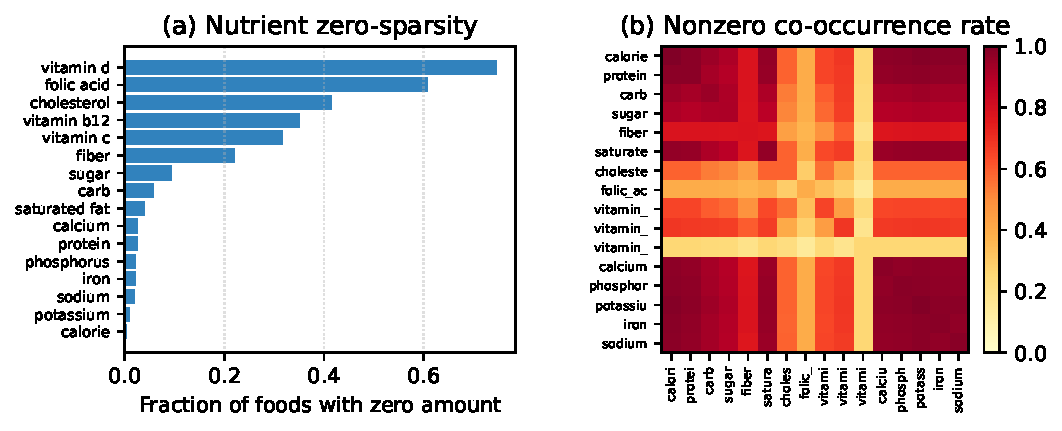
\includegraphics[width=\textwidth]{fig_s1_nutrient_sparsity.pdf}
\caption{NHANES nutrient sparsity diagnostics (unique-food subsample).
(a)~Fraction of foods with a zero amount for each nutrient.
(b)~Pairwise rate at which two nutrients are simultaneously nonzero in the same food.
High zero-sparsity and structured co-occurrence help explain why tight multi-nutrient interval boxes
induce sparse feasible assemblies under binary subset selection.}
\label{fig:s1}
\end{figure}

\clearpage
\section{Part B: Complete Algorithm Configuration Sheets}
\label{sec:sb}

Table~\ref{tab:s3} expands the compressed operator sheet of the main manuscript.
All solvers share the PRIMARY budget cell; RVEA and C-TAEA are invoked through \texttt{pymoo}~$0.6.x$
(local environment: $0.6.2$), which is the disclosed implementation-path asymmetry discussed in the fairness audit.

\begin{table}[!t]
\centering
\caption{Full PRIMARY configuration sheet.
SBX/PM settings follow the repository's pymoo wrappers ($\eta_c=15$, $\eta_m=20$, $p_c=0.9$, $p_m=1.0$ with RoundingRepair),
not a generic continuous MOEA default of $\eta_c=20$ / $p_m=1/n$.
Memetic local search follows Algorithm~1 of the main manuscript.}
\label{tab:s3}
\scriptsize
\setlength{\tabcolsep}{3pt}
\begin{tabular}{@{}llp{10cm}@{}}
\toprule
Algorithm & Family & Detailed configuration \\
\midrule
MA & Memetic / feas.-biased & Population $500$; set/swap crossover $p_c=0.2$; add/delete/replace mutation $p_m=0.9$;
CV-reducing local search on offspring (greedy add/swap within a capped inner evaluation budget; contributes to the
documented $\approx$100.8k median $n_{\mathrm{evals}}$ residual). \\
ACMO-Diet & Constrained MO + repair & Feasibility-biased selection; repair intensifications; memetic local improvement;
PRIMARY decode identical to other RCFA solvers~\cite{zhao2025acmodiet}. \\
BMOEA & Feas.-biased EA & Set-union subsample crossover $0.2$; add/delete/replace mutation $0.9$;
feasibility-first population rebuild; no separate LS loop. \\
NSGA-II & Dominance MOEA & pymoo NSGA-II; SBX ($p_c=0.9$, $\eta_c=15$); PM ($p_m=1.0$, $\eta_m=20$);
RoundingRepair on integer padded encoding; $n_{\mathrm{constr}}=0$ soft-penalty bi-objective~\cite{deb2002}. \\
SPEA2 & Indicator/archive & Same SBX/PM/RoundingRepair stack; external archive truncation~\cite{zitzler2001}. \\
RVEA & Reference-vector & Same variation stack; Das--Dennis-style reference directions via pymoo;
angle-penalized environmental selection~\cite{cheng2016}. \\
C-TAEA & Constrained two-archive & Same variation stack; CA/DA archives via pymoo CTAEA;
PRIMARY still uses soft bi-objective decode ($n_{\mathrm{constr}}=0$), a disclosed mechanism--implementation coupling~\cite{li2019ctaea}. \\
Greedy & Constructive heuristic & Nutrient-deficit scoring fill; candidate scoring may slightly overshoot the ceiling
(median $\approx$100.2k). \\
RandomRepair & Repair baseline & Random assemblies + delete upper violators / add deficit foods; $\le 20$ repair steps per sample;
continues until the shared $100$k evaluation ceiling. \\
Random & Unstructured baseline & Uniform cardinality-feasible sampling without repair or bias. \\
\bottomrule
\end{tabular}
\end{table}

\clearpage
\section{Part C: Exhaustive Cell-by-Cell FHR Results}
\label{sec:sc}

Tables~\ref{tab:s4}--\ref{tab:s6} list seed-level mean$\pm$std FHR for every PRIMARY cell underlying
the E1--E3 trend plots of the main manuscript.
These matrices allow a reviewer to verify any single cell without re-running solvers.
Two reading notes:
(i)~Recipe ceilings in Table~\ref{tab:s4} are identically $1.000$ and must not be used for ranking;
(ii)~E2 gaps in Table~\ref{tab:s5} are absolute FHR lifts, not rank changes---rank concordance is reserved for E4 / Part~D.

\begin{table}[!t]
\centering
\caption{E1 full scale sweep (seed-level mean$\pm$std FHR).
Recipe rows are a perfect ceiling ($\mathrm{FHR}=1.000$ for every solver) and are excluded from ranking aggregates
in the main manuscript. NHANES scales use the matched interval construction.}
\label{tab:s4}
\scriptsize
\setlength{\tabcolsep}{2.2pt}
\resizebox{\textwidth}{!}{\begin{tabular}{@{}lcccccccccc@{}}
\toprule
Scale & MA & ACMO & NSGA-II & BMOEA & SPEA2 & Repair & RVEA & C-TAEA & Greedy & Random \\
\midrule
Recipe & $\mathbf{1.000}$ & $\mathbf{1.000}$ & $\mathbf{1.000}$ & $\mathbf{1.000}$ & $\mathbf{1.000}$ & $\mathbf{1.000}$ & $\mathbf{1.000}$ & $\mathbf{1.000}$ & $\mathbf{1.000}$ & $\mathbf{1.000}$ \\
\midrule
5K & 0.967$\pm$0.043 & 0.983$\pm$0.035 & 0.992$\pm$0.026 & 0.958$\pm$0.059 & 0.917$\pm$0.056 & 0.817$\pm$0.095 & 0.750$\pm$0.096 & 0.567$\pm$0.117 & 0.575$\pm$0.107 & 0.325$\pm$0.061 \\
10K & $\mathbf{1.000}$ & 0.950$\pm$0.058 & 0.933$\pm$0.077 & 0.975$\pm$0.040 & 0.858$\pm$0.079 & 0.742$\pm$0.061 & 0.733$\pm$0.102 & 0.542$\pm$0.081 & 0.508$\pm$0.073 & 0.325$\pm$0.047 \\
25K & 0.975$\pm$0.040 & 0.992$\pm$0.026 & 0.975$\pm$0.040 & 0.950$\pm$0.043 & 0.892$\pm$0.069 & 0.925$\pm$0.061 & 0.842$\pm$0.127 & 0.608$\pm$0.111 & 0.658$\pm$0.061 & 0.417$\pm$0.056 \\
50K & 0.967$\pm$0.058 & 0.975$\pm$0.040 & 0.883$\pm$0.058 & 0.933$\pm$0.053 & 0.858$\pm$0.079 & 0.792$\pm$0.059 & 0.775$\pm$0.088 & 0.558$\pm$0.056 & 0.600$\pm$0.053 & 0.342$\pm$0.047 \\
100K & 0.983$\pm$0.035 & 0.950$\pm$0.043 & 0.942$\pm$0.056 & 0.958$\pm$0.071 & 0.850$\pm$0.102 & 0.800$\pm$0.070 & 0.825$\pm$0.083 & 0.617$\pm$0.081 & 0.600$\pm$0.077 & 0.325$\pm$0.026 \\
$\approx$210K & 0.983$\pm$0.035 & 0.975$\pm$0.040 & 0.950$\pm$0.058 & 0.983$\pm$0.035 & 0.833$\pm$0.088 & 0.858$\pm$0.056 & 0.867$\pm$0.098 & 0.558$\pm$0.097 & 0.608$\pm$0.088 & 0.333$\pm$0.056 \\
\bottomrule
\end{tabular}}
\end{table}

\begin{table}[!t]
\centering
\caption{E2 full sparsity sweep (seed-level mean$\pm$std FHR) on NHANES-10K.
The final row reports the absolute FHR lift from $f=0.5$ to $f=1.5$ for each solver,
quantifying the ``nearly an order of magnitude'' difficulty shift emphasized in the main manuscript.}
\label{tab:s5}
\scriptsize
\setlength{\tabcolsep}{2.2pt}
\resizebox{\textwidth}{!}{\begin{tabular}{@{}lccccccccccc@{}}
\toprule
$f$ & MA & ACMO & NSGA-II & BMOEA & SPEA2 & Repair & RVEA & C-TAEA & Greedy & Random & Mean gap \\
\midrule
0.5 & 0.275$\pm$0.056 & 0.217$\pm$0.043 & 0.217$\pm$0.058 & 0.192$\pm$0.040 & 0.183$\pm$0.035 & 0.242$\pm$0.026 & 0.158$\pm$0.026 & 0.108$\pm$0.040 & 0.108$\pm$0.040 & 0.017$\pm$0.035 & --- \\
1.0 & 0.992$\pm$0.026 & 0.975$\pm$0.040 & 0.967$\pm$0.058 & 0.933$\pm$0.053 & 0.850$\pm$0.102 & 0.750$\pm$0.088 & 0.767$\pm$0.117 & 0.517$\pm$0.110 & 0.550$\pm$0.098 & 0.308$\pm$0.040 & --- \\
1.5 & $\mathbf{1.000}$ & $\mathbf{1.000}$ & $\mathbf{1.000}$ & $\mathbf{1.000}$ & 0.983$\pm$0.035 & $\mathbf{1.000}$ & 0.950$\pm$0.070 & 0.925$\pm$0.083 & 0.917$\pm$0.000 & 0.850$\pm$0.066 & 0.791 \\
\midrule
$1.5{-}0.5$ & 0.725 & 0.783 & 0.783 & 0.808 & 0.800 & 0.758 & 0.792 & 0.817 & 0.808 & 0.833 & --- \\
\bottomrule
\end{tabular}}
\end{table}

\begin{table}[!t]
\centering
\caption{E3 full dimension sweep (seed-level mean$\pm$std FHR) on NHANES-10K.
Boldface marks the best mean in each row.
Low dimensions sit near ceiling; dimension~$16$ exposes selective degradation of weaker solvers.}
\label{tab:s6}
\scriptsize
\setlength{\tabcolsep}{2.5pt}
\resizebox{\textwidth}{!}{\begin{tabular}{@{}lcccccccc@{}}
\toprule
Dim & MA & ACMO & NSGA-II & BMOEA & SPEA2 & RVEA & C-TAEA & Random \\
\midrule
6 & \textbf{$\mathbf{1.000}$} & \textbf{$\mathbf{1.000}$} & \textbf{$\mathbf{1.000}$} & \textbf{$\mathbf{1.000}$} & \textbf{$\mathbf{1.000}$} & \textbf{$\mathbf{1.000}$} & 0.983$\pm$0.035 & 0.950$\pm$0.043 \\
9 & \textbf{$\mathbf{1.000}$} & \textbf{$\mathbf{1.000}$} & \textbf{$\mathbf{1.000}$} & 0.992$\pm$0.026 & \textbf{$\mathbf{1.000}$} & 0.992$\pm$0.026 & 0.925$\pm$0.047 & 0.958$\pm$0.059 \\
12 & 0.992$\pm$0.026 & \textbf{$\mathbf{1.000}$} & \textbf{$\mathbf{1.000}$} & 0.992$\pm$0.026 & 0.967$\pm$0.043 & 0.983$\pm$0.035 & 0.850$\pm$0.053 & 0.783$\pm$0.070 \\
16 & \textbf{$\mathbf{1.000}$} & 0.975$\pm$0.040 & 0.958$\pm$0.044 & 0.983$\pm$0.035 & 0.817$\pm$0.077 & 0.733$\pm$0.066 & 0.592$\pm$0.127 & 0.300$\pm$0.043 \\
\bottomrule
\end{tabular}}
\end{table}

\clearpage
\section{Part D: Post-hoc Pairwise Significance Tests}
\label{sec:sd}

Friedman $p$-values in the main manuscript establish global rank differences but do not identify which pairs drive significance.
Tables~\ref{tab:s7}--\ref{tab:s8} supply pairwise Wilcoxon signed-rank outcomes
($+$: row significantly higher FHR than column at $p\le 0.05$;
$-$: significantly lower; $\approx$: not significant).
Tests are paired by $(\mathrm{target},\mathrm{seed})$.
Exact two-sided $p$-values are printed as non-floating panels beneath Tables~\ref{tab:s7}--\ref{tab:s8}
(and archived as CSV beside the build-script outputs).

\paragraph{How to read the E2 ($f=0.5$) matrix.}
The top-tier pattern is visible without crowning a champion:
MA beats Random and several mid/low solvers, yet remains statistically tied with NSGA-II at the $0.05$ threshold ($p\approx 0.052$).
RandomRepair remains competitive against several structured solvers under this sparse cell, reinforcing that repair pressure---not merely metaheuristic branding---matters when the box is tight.

\paragraph{How to read the E3 (dim~$16$) matrix.}
Selective degradation appears as a block of ``$-$'' entries from weaker solvers toward the top tier, while MA/ACMO/BMOEA stay mutually close.
This is the pairwise counterpart of the main-manuscript claim that high dimensionality hurts unevenly.

\begin{table}[!t]
\centering
\caption{Pairwise Wilcoxon signed-rank matrix for E2 hardest cell ($f=0.5$).
Reading the MA row: MA is significantly above Random/C-TAEA/Greedy/RVEA/SPEA2/BMOEA,
but \emph{not} significantly separated from NSGA-II or RandomRepair at $p\le 0.05$
(MA vs.\ NSGA-II $p\approx 0.052$).
This pattern supports stable top-tier membership rather than a single universal champion.}
\label{tab:s7}
\scriptsize
\begin{tabular}{@{}lcccccccccc@{}}
\toprule
 & MA & ACMO & NSGA-II & BMOEA & SPEA2 & Repair & RVEA & C-TAEA & Greedy & Random \\
\midrule
MA & --- & + & $\approx$ & + & + & $\approx$ & + & + & + & + \\
ACMO & - & --- & $\approx$ & $\approx$ & $\approx$ & $\approx$ & + & + & + & + \\
NSGA-II & $\approx$ & $\approx$ & --- & $\approx$ & $\approx$ & $\approx$ & + & + & + & + \\
BMOEA & - & $\approx$ & $\approx$ & --- & $\approx$ & - & + & + & + & + \\
SPEA2 & - & $\approx$ & $\approx$ & $\approx$ & --- & - & $\approx$ & + & + & + \\
Repair & $\approx$ & $\approx$ & $\approx$ & + & + & --- & + & + & + & + \\
RVEA & - & - & - & - & $\approx$ & - & --- & $\approx$ & + & + \\
C-TAEA & - & - & - & - & - & - & $\approx$ & --- & $\approx$ & + \\
Greedy & - & - & - & - & - & - & - & $\approx$ & --- & + \\
Random & - & - & - & - & - & - & - & - & - & --- \\
\bottomrule
\end{tabular}
\end{table}

\begin{table}[!t]
\centering
\caption{Pairwise Wilcoxon signed-rank matrix for E3 dimension~$16$.
Leading memetic/dominance solvers remain mutually close ($\approx$ among MA/ACMO/BMOEA),
while Random and C-TAEA are significantly below the top tier---consistent with selective high-dimensional degradation.}
\label{tab:s8}
\scriptsize
\begin{tabular}{@{}lcccccccc@{}}
\toprule
 & MA & ACMO & NSGA-II & BMOEA & SPEA2 & RVEA & C-TAEA & Random \\
\midrule
MA & --- & $\approx$ & + & $\approx$ & + & + & + & + \\
ACMO & $\approx$ & --- & $\approx$ & $\approx$ & + & + & + & + \\
NSGA-II & - & $\approx$ & --- & $\approx$ & + & + & + & + \\
BMOEA & $\approx$ & $\approx$ & $\approx$ & --- & + & + & + & + \\
SPEA2 & - & - & - & - & --- & $\approx$ & + & + \\
RVEA & - & - & - & - & $\approx$ & --- & + & + \\
C-TAEA & - & - & - & - & - & - & --- & + \\
Random & - & - & - & - & - & - & - & --- \\
\bottomrule
\end{tabular}
\end{table}

\noindent\textbf{$p$-values for Table~\ref{tab:s7} (E2, $f=0.5$).}\\[0.3em]
{\centering\scriptsize\resizebox{\textwidth}{!}{\begin{tabular}{@{}lcccccccccc@{}}
\toprule
 & MA & ACMO & NSGA-II & BMOEA & SPEA2 & Repair & RVEA & C-TAEA & Greedy & Random \\
\midrule
MA & --- & 0.035 & 0.052 & 0.012 & 9.1e-04 & 0.206 & 1.8e-04 & 7.7e-06 & 7.7e-06 & 2.6e-08 \\
ACMO & 0.035 & --- & 1.000 & 0.317 & 0.102 & 0.257 & 0.008 & 3.1e-04 & 3.1e-04 & 9.6e-07 \\
NSGA-II & 0.052 & 1.000 & --- & 0.257 & 0.102 & 0.257 & 0.008 & 3.1e-04 & 3.1e-04 & 9.6e-07 \\
BMOEA & 0.012 & 0.317 & 0.257 & --- & 0.655 & 0.034 & 0.046 & 0.004 & 0.002 & 4.6e-06 \\
SPEA2 & 9.1e-04 & 0.102 & 0.102 & 0.655 & --- & 0.008 & 0.083 & 0.003 & 0.003 & 7.7e-06 \\
Repair & 0.206 & 0.257 & 0.257 & 0.034 & 0.008 & --- & 0.002 & 6.3e-05 & 6.3e-05 & 2.0e-07 \\
RVEA & 1.8e-04 & 0.008 & 0.008 & 0.046 & 0.083 & 0.002 & --- & 0.058 & 0.034 & 9.6e-05 \\
C-TAEA & 7.7e-06 & 3.1e-04 & 3.1e-04 & 0.004 & 0.003 & 6.3e-05 & 0.058 & --- & 1.000 & 9.1e-04 \\
Greedy & 7.7e-06 & 3.1e-04 & 3.1e-04 & 0.002 & 0.003 & 6.3e-05 & 0.034 & 1.000 & --- & 9.1e-04 \\
Random & 2.6e-08 & 9.6e-07 & 9.6e-07 & 4.6e-06 & 7.7e-06 & 2.0e-07 & 9.6e-05 & 9.1e-04 & 9.1e-04 & --- \\
\bottomrule
\end{tabular}}\par}
\vspace{0.8em}
\noindent\textbf{$p$-values for Table~\ref{tab:s8} (E3, dimension~$16$).}\\[0.3em]
{\centering\scriptsize\resizebox{\textwidth}{!}{\begin{tabular}{@{}lcccccccc@{}}
\toprule
 & MA & ACMO & NSGA-II & BMOEA & SPEA2 & RVEA & C-TAEA & Random \\
\midrule
MA & --- & 0.083 & 0.025 & 0.157 & 2.7e-06 & 1.5e-08 & 2.6e-12 & 4.9e-20 \\
ACMO & 0.083 & --- & 0.414 & 0.655 & 3.4e-05 & 4.5e-07 & 3.1e-11 & 2.3e-19 \\
NSGA-II & 0.025 & 0.414 & --- & 0.257 & 3.9e-04 & 5.0e-06 & 2.1e-10 & 6.2e-19 \\
BMOEA & 0.157 & 0.655 & 0.257 & --- & 4.5e-05 & 2.7e-07 & 1.9e-11 & 9.4e-19 \\
SPEA2 & 2.7e-06 & 3.4e-05 & 3.9e-04 & 4.5e-05 & --- & 0.077 & 2.5e-05 & 9.2e-15 \\
RVEA & 1.5e-08 & 4.5e-07 & 5.0e-06 & 2.7e-07 & 0.077 & --- & 0.004 & 1.5e-12 \\
C-TAEA & 2.6e-12 & 3.1e-11 & 2.1e-10 & 1.9e-11 & 2.5e-05 & 0.004 & --- & 1.8e-07 \\
Random & 4.9e-20 & 2.3e-19 & 6.2e-19 & 9.4e-19 & 9.2e-15 & 1.5e-12 & 1.8e-07 & --- \\
\bottomrule
\end{tabular}}\par}

\clearpage
\section{Part E: Abandoned Exploratory Analysis --- Unstable $N^*$ Fits}
\label{sec:se}

Exploratory logistic fits of FHR versus $\log_{10} N$ on E1 NHANES scales do not yield a stable inflection $N^*$.
Figure~\ref{fig:s2} repeats the fit under four random target splits.
Inflection estimates drift over many orders of magnitude and frequently fail for top solvers with flat FHR curves.
These diagnostics motivated abandonment of any PRIMARY phase-transition / $N^*$ claim.

\begin{figure}[!t]
\centering
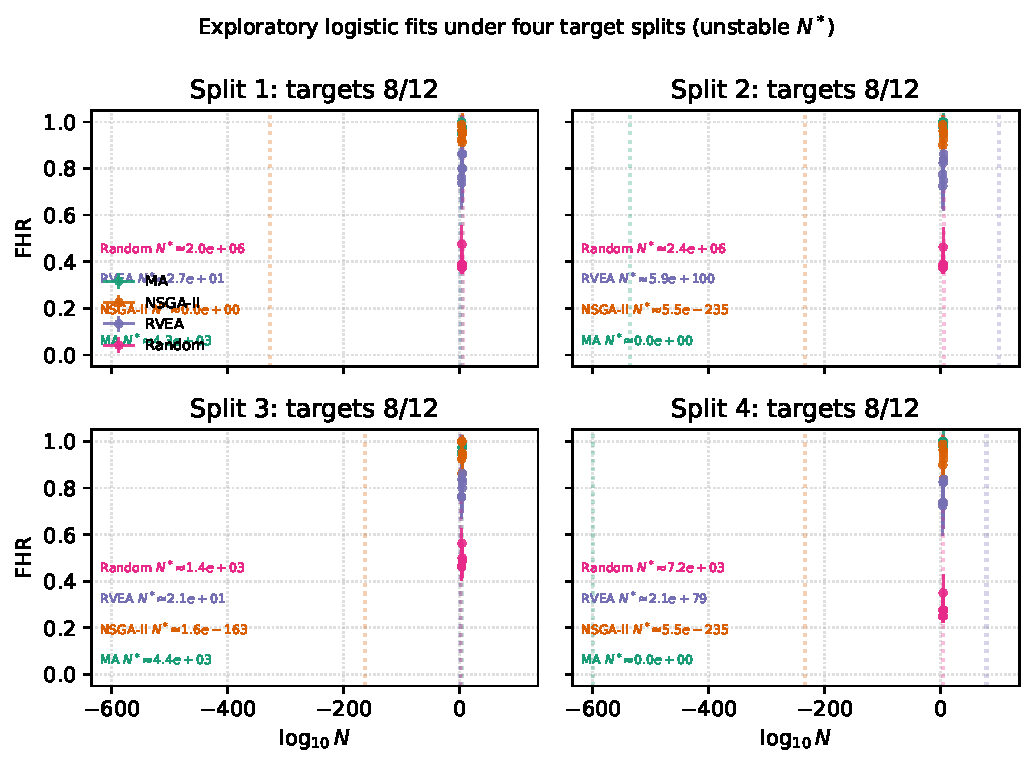
\includegraphics[width=\textwidth]{fig_s2_unstable_nstar.pdf}
\caption{Exploratory logistic fits for FHR vs.\ $\log_{10} N$ under four different target splits
(eight of twelve representatives resampled each panel).
Solid markers: observed seed-level mean$\pm$std.
Dashed curves: attempted logistic fits; vertical guides mark fitted $x_0=\log_{10} N^*$.
Wide disagreement of $N^*$ across splits and frequent fit failures illustrate why a scaling-law / phase-transition
narrative was not retained as a PRIMARY conclusion.}
\label{fig:s2}
\end{figure}

\clearpage
\section{Part F: Search Dynamics --- Evaluations to First Feasible}
\label{sec:sf}

Complementing the reconstructed CV trajectories in the main manuscript,
Fig.~\ref{fig:s3} reports evaluations to first feasible (FFG) on successful runs only for E2 $f=0.5$.
Random is omitted because it almost never hits under this cell (mean FHR $\approx 0.017$).
Hit counts and median FFG are printed beneath the panel.

\begin{figure}[!t]
\centering
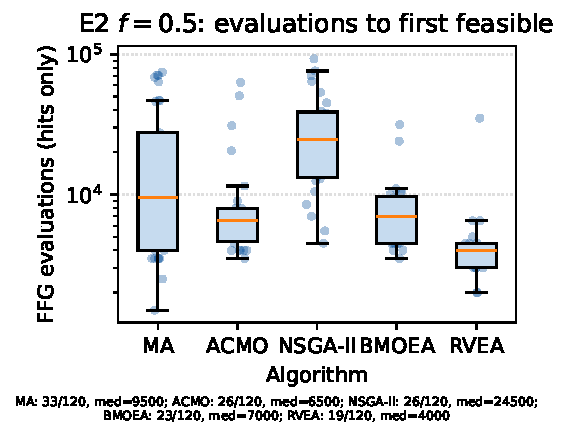
\includegraphics[width=\columnwidth]{fig_s3_ffg_first_hit.pdf}
\caption{E2 $f=0.5$: distribution of evaluations to first feasible among successful $(\mathrm{target},\mathrm{seed})$ runs
for five structured solvers (log scale).
Non-hits are excluded from the box/swarm (censored at $100$k in the raw CSV).
Random is omitted due to near-zero hit rate.
These diagnostics inform early-stopping practice but do not replace FHR as the PRIMARY success metric.}
\label{fig:s3}
\end{figure}

\clearpage
\section{Part G: Fairness Residuals and Budget Auditing}
\label{sec:sg}

Table~\ref{tab:s9} lists median realized evaluation counts by solver and campaign.
Most solvers sit exactly on the $100{,}000$ ceiling.
MA overshoots by $<0.83\%$ (local-search accounting); Greedy by $<0.20\%$.
RandomRepair matches the ceiling on PRIMARY E1/E2 after the under-budget repair fix documented in the fairness audit.
These residuals bound---rather than invalidate---the fair-budget claim of the main manuscript.

\begin{table}[!t]
\centering
\caption{Median realized $n_{\mathrm{evals}}$ by solver and campaign versus the theoretical ceiling of $100{,}000$.
E3 omits Greedy and RandomRepair by campaign design.}
\label{tab:s9}
\scriptsize
\begin{tabular}{@{}lccc@{}}
\toprule
Algorithm & E1 median $n_{\mathrm{evals}}$ & E2 & E3 \\
\midrule
Theoretical ceiling & 100000 & 100000 & 100000 \\
\midrule
MA & 100806 & 100808 & 100825 \\
ACMO & 100000 & 100000 & 100000 \\
NSGA-II & 100000 & 100000 & 100000 \\
BMOEA & 100000 & 100000 & 100000 \\
SPEA2 & 100000 & 100000 & 100000 \\
Repair & 100000 & 100000 & --- \\
RVEA & 100000 & 100000 & 100000 \\
C-TAEA & 100000 & 100000 & 100000 \\
Greedy & 100178 & 100191 & --- \\
Random & 100000 & 100000 & 100000 \\
\bottomrule
\end{tabular}
\end{table}

\section*{Reproducibility Pointers}
All numbers in this supplement are regenerated from
\texttt{results/raw/e\{1,2,3\}\_*\_full.csv} by \texttt{scripts/build\_supplement.py}.
Re-running that script refreshes Tables~S1--S9 and Figs.~S1--S3 without modifying PRIMARY solver outputs.
For code, environment fingerprints, and fairness notes, see the public GitHub repository and
\texttt{docs/FAIRNESS\_AUDIT.md}.

\begin{thebibliography}{5}
\bibitem{deb2002}
K.~Deb, A.~Pratap, S.~Agarwal, and T.~Meyarivan,
``A fast and elitist multiobjective genetic algorithm: NSGA-II,''
\emph{IEEE Trans. Evol. Comput.}, vol.~6, no.~2, pp.~182--197, 2002.
\bibitem{zitzler2001}
E.~Zitzler, M.~Laumanns, and L.~Thiele,
``SPEA2: Improving the strength Pareto evolutionary algorithm,''
\emph{TIK-Report}, vol.~103, 2001.
\bibitem{cheng2016}
R.~Cheng, Y.~Jin, M.~Olhofer, and B.~Sendhoff,
``A reference vector guided evolutionary algorithm for many-objective optimization,''
\emph{IEEE Trans. Evol. Comput.}, vol.~20, no.~5, pp.~773--791, 2016.
\bibitem{li2019ctaea}
K.~Li, R.~Chen, G.~Fu, and X.~Yao,
``Two-archive evolutionary algorithm for constrained multiobjective optimization,''
\emph{IEEE Trans. Evol. Comput.}, vol.~23, no.~2, pp.~303--315, 2019.
\bibitem{zhao2025acmodiet}
L.~Zhao et~al.,
``ACMO-Diet,'' companion method cited in the main manuscript bibliography.
\end{thebibliography}

\end{document}
